%\section{The CMS Experiment}

The Compact Muon Solenoid (CMS) detector is a general purpose particle detector designed to investigate various physical phenomena concerning the SM and beyond it, such as Supersymmetry, Extra Dimensions and Dark Matter. As its name implies, the detector is a solenoid which is  constructed around a superconducting magnet capable of producing a magnetic field of 3.8 T. The magnetic coil is 13m long with an inner diameter of 6m, making it the largest superconducting magnet ever constructed. The CMS detector itself is 21m long with a diameter of 15m and it has a weight of approximately 14,000 tons. The CMS experiment is one of the largest scientific collaborations in the history of mankind with over 4,000 participants from 42 countries and 182 institutions. CMS is located at one of these points and it essentially acts as a giant super highspeed camera that makes 3D images of the collisions that are produced at a rate of 40 MHz (40 million times per second). The detector has an onion-like structure to capture all the particles that are produced in these high energy collisions most of them being unstable and decaying further to stable particles that are detected.  CMS detector was designed with the following features (as shown in \autoref{test}) :

\begin{enumerate}
	\item{A \textbf{magnet} with large bending power and high performance muon detector for good muon
identification and momentum resolution over a wide range of momenta and angles.}

	\item{An \textbf{inner tracking system} capable of high reconstruction efficiency and momentum resolution
requiring \textbf{pixel detectors} close to the interaction region.}

	\item{An \textbf{electromagnetic calorimeter} able to provide good electromagnetic energy resolution and  
a high isolation efficiency for photons and leptons.}

	\item{A \textbf{hadron calorimeter} capable of providing precise missing-transverse-energy and dijet-mass  
resolution.}

\end{enumerate}

\begin{figure}
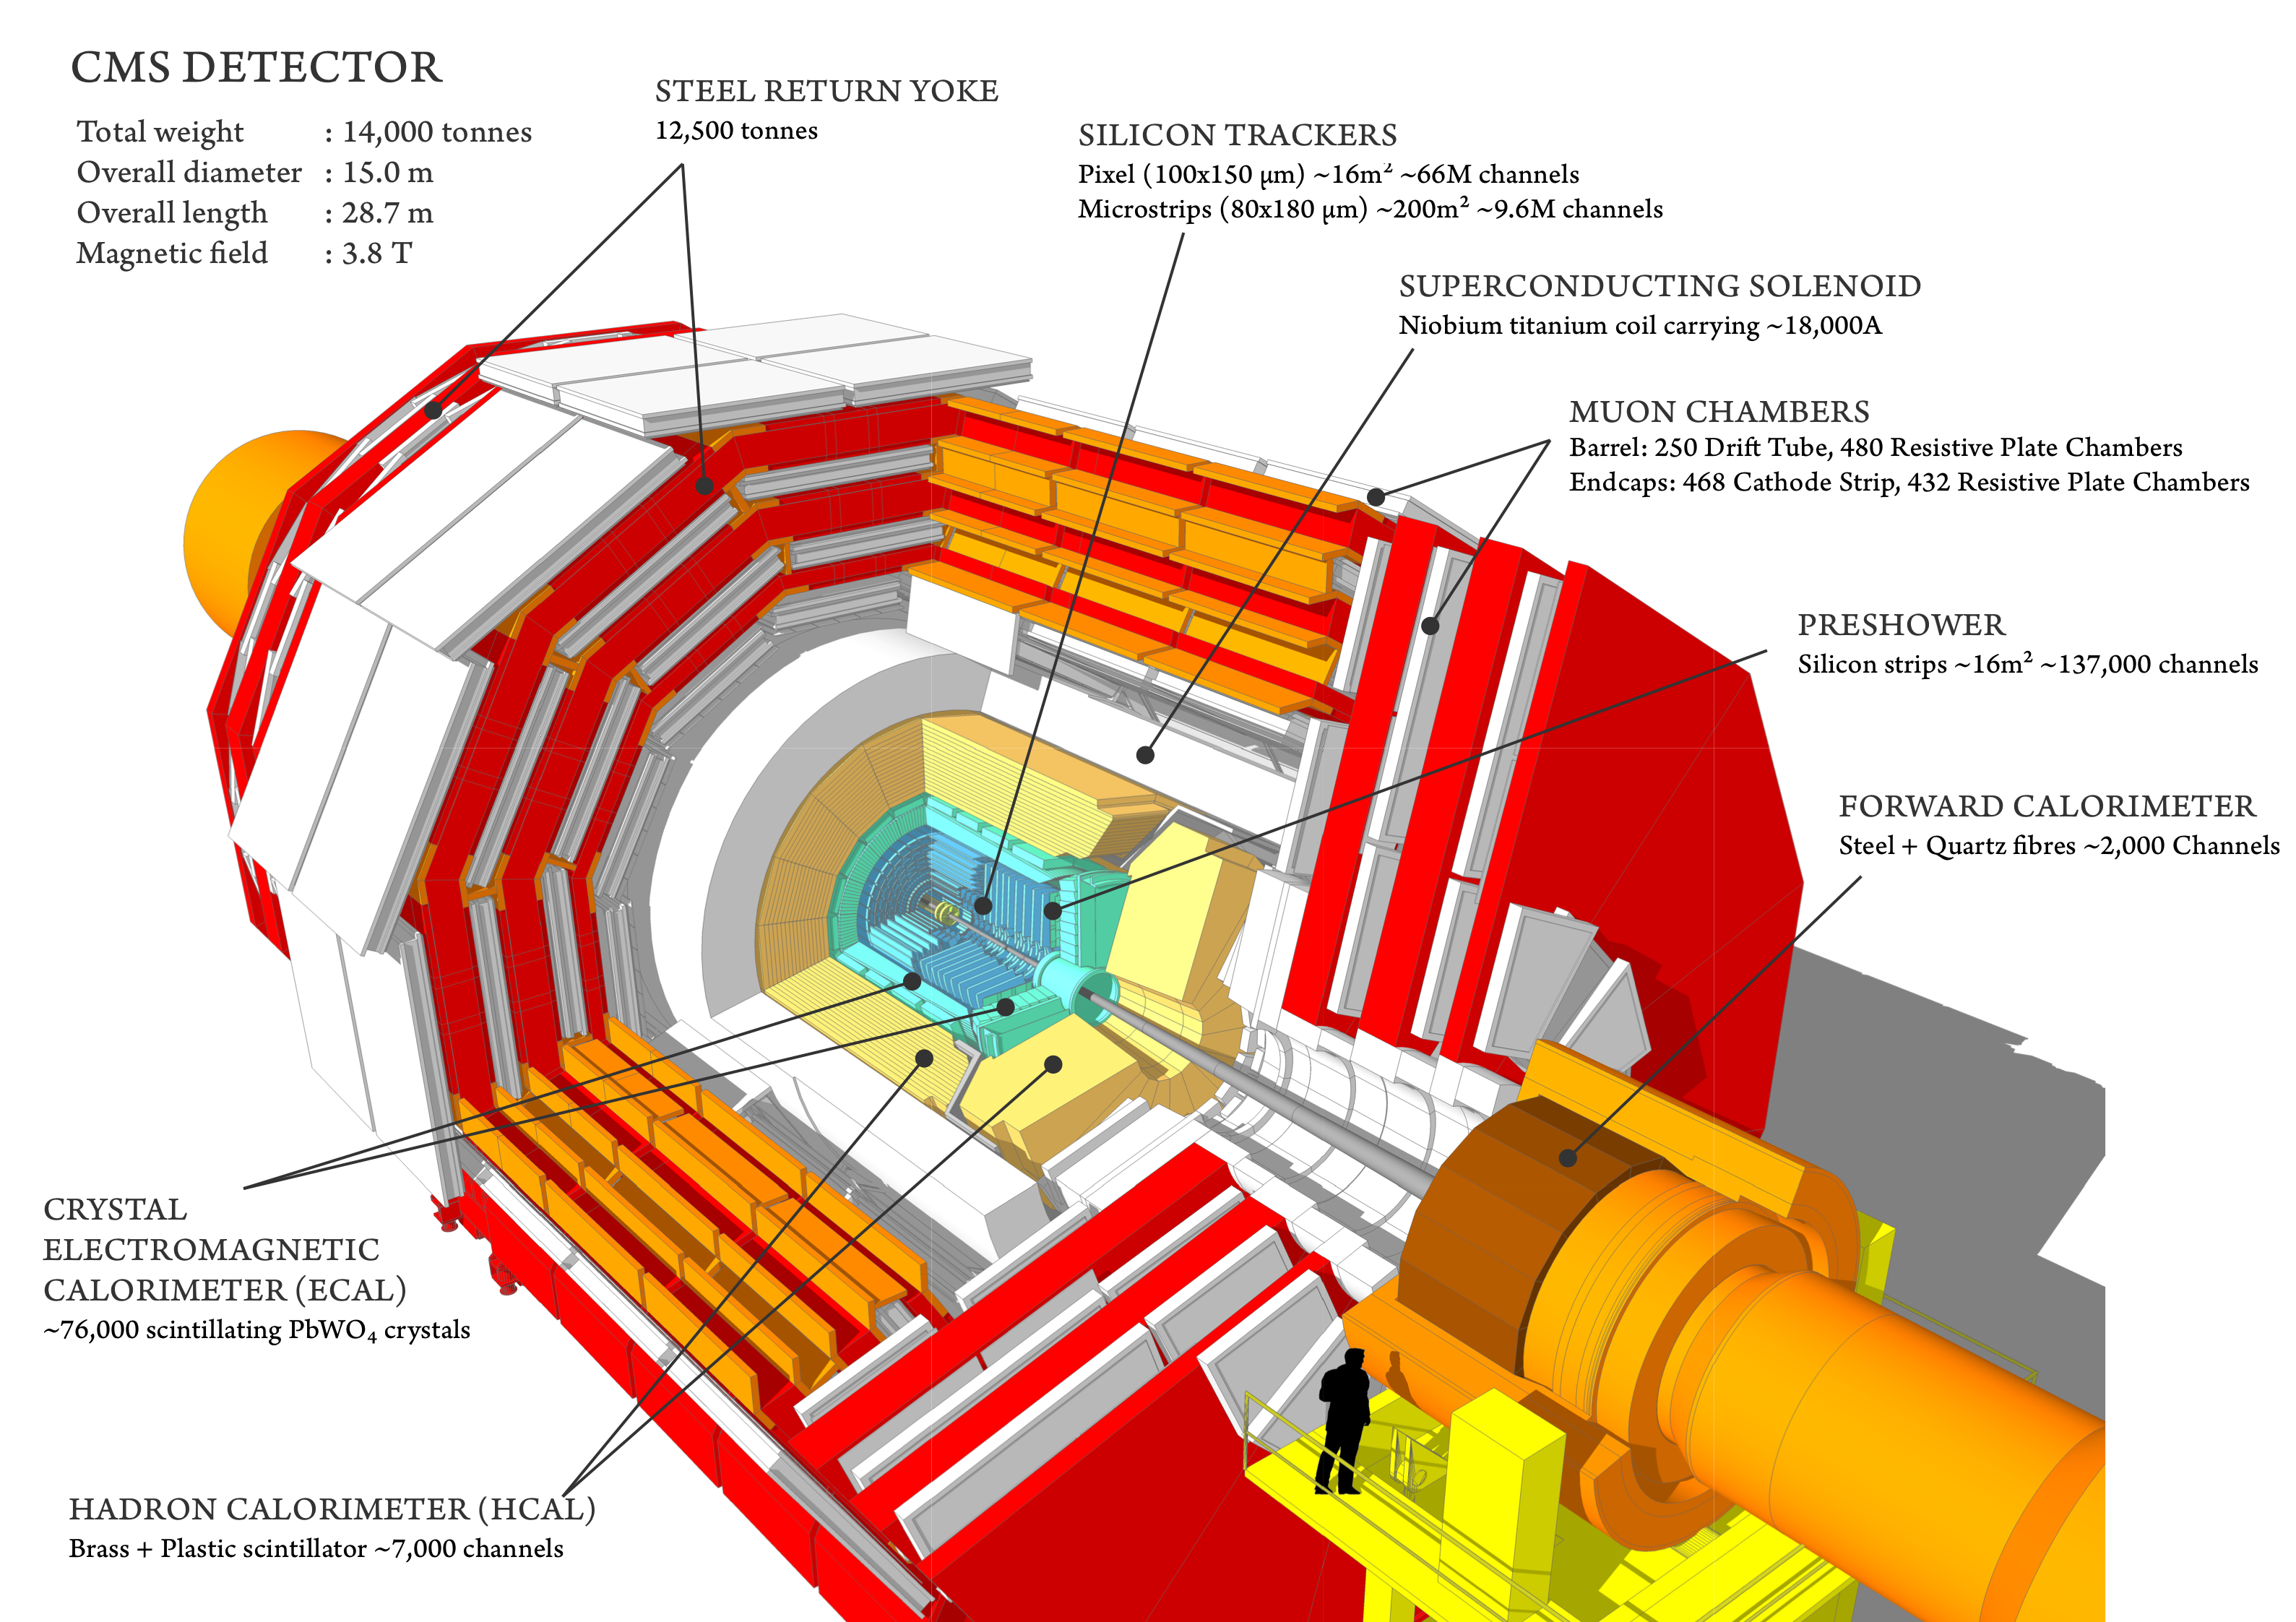
\includegraphics[width=\linewidth]{CMSLayout.png}
\label{Guillermo}
\caption{CMS Detector \label{test}}
\end{figure}

A property from these particles that is exploited is their charge. Normally, particles produced in collisions travel in a straight line, but in the presence of a magnetic field, their paths are skewed and curved. Except the muon system, the rest of the subdetectors lie inside a 3.8 Tesla magnetic field . Due to the magnetic field the trajectory of charged particle produced in the collisions gets curved  (as shown in \autoref{Guillermo} ) and one can calculate the particle’s momentum and know the type of charge on the particle.  The Tracking devices are responsible for drawing the trajectory of the particles by using a computer program that reconstructs the path by using electrical signals that are left by the particle as they move.  The Calorimeters measure the energy of particles that pass through them by absorbing their energy with the intent of stopping them. The particle identification detectors work by detecting radiation emitted by charged particles and using this information they can measure the speed, momentum, and mass of a particle. After the information is put together to make the “snapshot” of the collision one looks for results that do not fit the current theories or models in order to look for new physics.

\begin{figure}
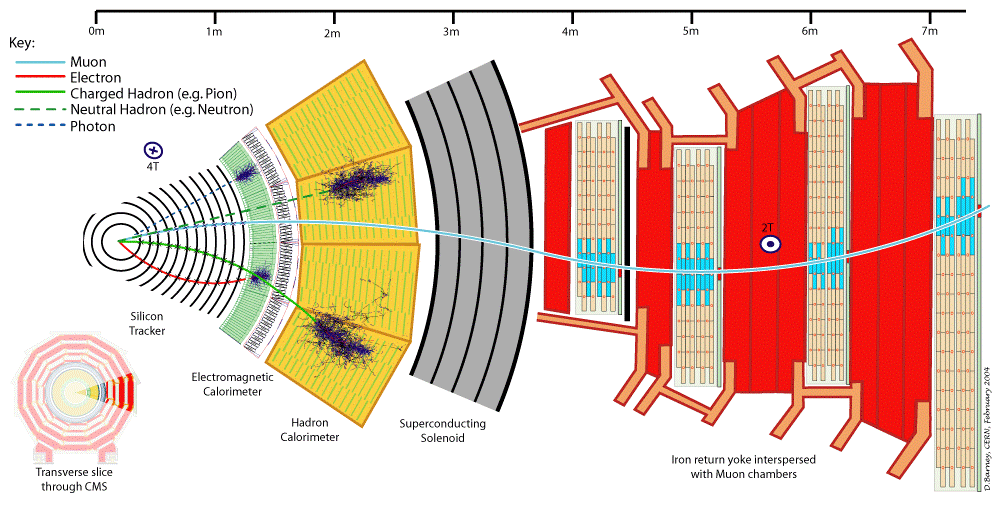
\includegraphics[width=\linewidth]{CMSLayers.PNG}
\label{CMSLayers}
\caption{The trajectory of a particle traveling through the layers of the detector leaving behind a it's signature footprint}
\end{figure}


\section{Supersymmetric extension of the Standard Model}

The supersymmetry theories are based on a symmetry between fermions and bosons. It is similar to solving the `electron mass hierarchy problem' in quantum mechanics, where the number of particles is doubled: in addition to the electron, there is also a positron. The virtual electron--positron contributions solved the problem of electrons having a small mass by smearing out the electric charge. Supersymmetry is an analogous theory where once again the set of particles is doubled, and in doing so the loop contributions of one particle to the Higgs are cancelled by the loop contributions of its super-partner. It extends space-time symmetry since it relates matter particles to force particles. It relates particles with different spins but the same gauge charges.\autoref{CMSLayers}

\begin{figure}[H]
\begin{center}
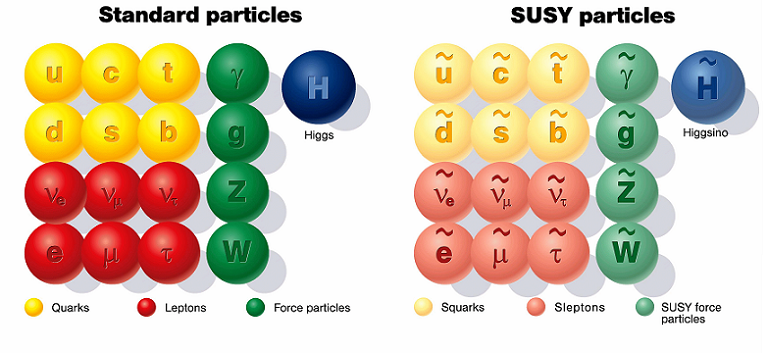
\includegraphics[width=0.9\textwidth]{SUSY.png} 
\caption[Schematic representation of the Standard Model particles with the added SUSY particles.]{Schematic representation of the Standard Model particles with the added SUSY particles.}
\label{SUSY} 
%\hspace{4em}
\end{center}
\end{figure}

The gluon (QCD) has a fermionic partner, the gluino. Similarly, the spin 1 gauge bosons W+, W0, W- and B$^0$ have their counterparts, called winos and binos, that, after electroweak symmetry breaking, mix to give the mass eigenstate Z$^0$ and $\gamma$, and the zino and photino respectively. For every lepton/quark there is a bosonic partner (i.e. a scalar slepton/squark). There are three families for each of the quark and lepton supermultiplets. The left-handed and right-handed pieces of the squarks and sleptons are two separate components, as in the corresponding SM sector. The Higgs doublet is extended by another doublet leading to other Higgs boson particles (Higgsinos).\\

Even though supersymmetry solves many problems in particle physics, it also poses new problems. If these new particles had the same mass as their counterparts in the standard model, we would have already observed them. Since none of these particles have been found yet, SUSY must be a broken symmetry. What makes superpartners heavier than ordinary particles? Why are superpartners so well hidden in rare phenomena? This arbitrary mass spectrum for the superpartners would have effects that are far too large in rare processes that change the flavor of particles. There must be some special reason why such effects are well hidden. How do we extract information on the mechanism of supersymmetry breaking? How does supersymmetry impact cosmology? Is the lightest supersymmetric partner what really composes Dark Matter? Different mechanisms have been suggested on how this symmetry is broken and have led to different phenomenological scenarios like the minimal supergravity model (mSUGRA)\cite{mSugra1,mSugra2}, the gauge-mediated supersymmetry breaking (GMSB)\cite{GMSB1,GMSB2,GMSB3} model or R-parity\cite{Rparity1,Rparity2}. A discussion of mSUGRA and GMSB is beyond the scope of this dissertation. R-parity is a new symmetry that has been added to the minimal supersymmetry scenario which prevents the violation of the leptonic and baryonic numbers. All SM fields have even R-parity, while SUSY particles have odd R-parity. The most obvious experimental constraint comes from the non-observation of proton decay \cite{pDecay1}, which would violate both baryonic and leptonic number conservation. Due to R-parity every interaction vertex in the theory involves an even number of sparticles, meaning that they must be pair-produced. The decay chains of the produced particles are characterized by the presence of one stable particle, generically called the Lightest Supersymmetric Particle (LSP), that may account for all the dark matter in the Universe. However, in other models, like the R-parity violating SUSY this may not apply. In other scenarios, those LSP can be regarded as vanishing mass and may not be enough to satisfy the dark matter in the Universe.

\subsection{Simplified Models Approach to Supersymmetry}

Simplified models \cite{SSM} are a new approach for characterizing LHC supersymmetry results. In a simplified model only a few new particles and a single decay topology are introduced, and hence these models are easy to constrain. Traditionally, testing a particle physics theory against experimental results requires calculating what the theory predicts in an experimental situation using a particle accelerator detector. This translates into computing: the masses of new particles, their decay widths, their branching ratios and production cross-sections. This information is subsequently used in Monte Carlo simulations of passage of proton-proton collisions products and their decays through the CMS detector. This is done under the hypothesis that the theory is true. The simulated data is  analyzed just like the actual experimental data resulting from proton-proton collisions. The theoretical and the experimental results can then be compared. Though conceptually uncomplicated it requires access to the experimental data, and the step of simulating the detector response requires intimate knowledge of the CMS detector by theorist community. It is also restrictive being model/theory dependent. The CMS collaboration, like ATLAS, does not share experimental details but only the final results via publications. The Simplified Model approach circumvents this issue by presenting results on very simple phenomenological models instead of a specific model, such as the constrained MSSM (cMSSM) \cite{cMSSM}. Each simplified models encompasses a specific phenomenological feature that is common to many different theories. A limited set of hypothetical particles and decay chains are introduced to produce a given topological signature. The amplitudes describing the production and decays of these particles are parametrized in terms of the particle masses and their branching ratios to daughter particles. This makes the analysis of simplified models less model dependent. The Simplified Models assume that a particular decay signature can be realized without specifying the exact mechanism, offering the possibility to overcome small branching ratios. Some Simplified Models with their corresponding production and decay modes are shown in the \autoref{topologyTable}. We have used T2tt, T1tttt, T1ttbb, T5tttt and T5ttcc models in analysis in this thesis. Some of these topologies are further discussed in more detail in \autoref{AnalysisChap}, since they correspond to some of the signals for SUSY in the treated analysis.

\begin{table}[H]
\begin{center}
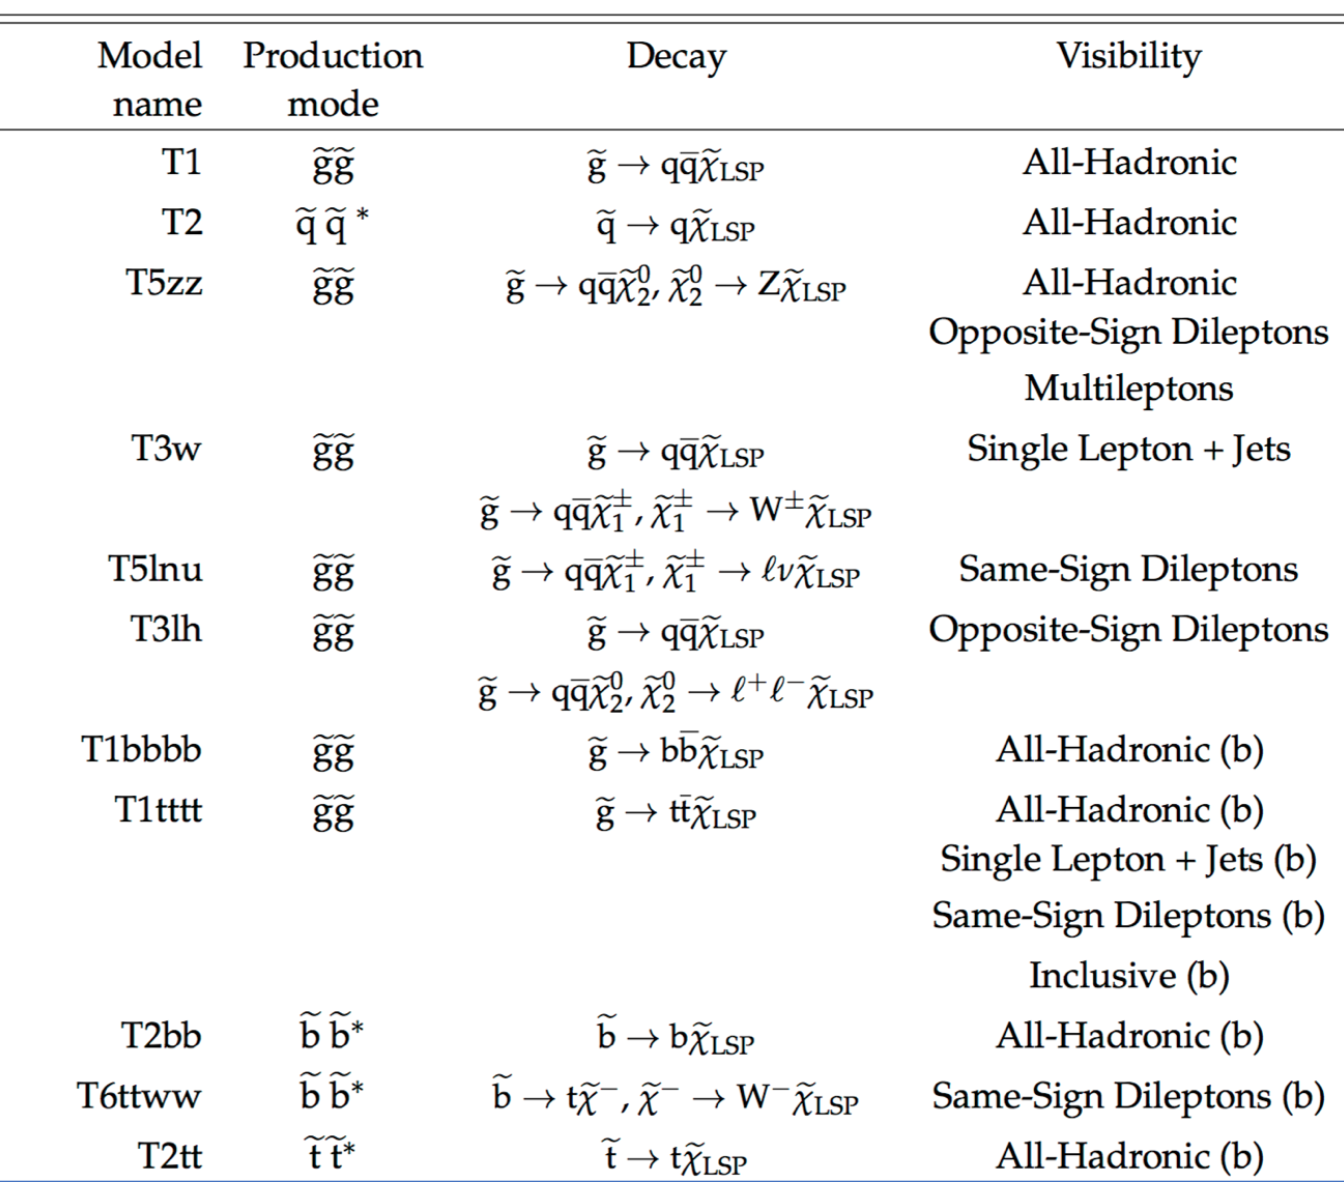
\includegraphics[width=0.9\textwidth]{topologyTable.png}
\caption{Some Simplified Models with their corresponding production and decay modes.}
\label{topologyTable}
\end{center}
\end{table}


